\documentclass[10pt]{report}

\usepackage[utf8]{inputenc} % Required for inputting international characters
\usepackage[T1]{fontenc} % Output font encoding for international characters
\usepackage[demo]{graphicx} % images % get rid of [demo] for black box removal
% \usepackage{graphicx} % images % get rid of [demo] for black box removal
\usepackage{fancyhdr} % headers and footers
% \usepackage{parskip} % paragraph
\usepackage{geometry} % page size
% \usepackage{hyperref} % Links
% \usepackage{pdflscape} % making a page landscape
\usepackage{xcolor}
\usepackage[shortlabels]{enumitem}
\usepackage{multirow}
\usepackage{listings}
\usepackage{titlesec}
\usepackage{float} % to place figures in place

\graphicspath{{../images/}}

\titleformat{\chapter}[display]
  {\normalfont\bfseries}{}{0pt}{\Huge}

% margins and page size
\geometry{
a4paper,
left=30mm,
top=25mm,
right=30mm,
bottom=25mm
}

\lstset{
  basicstyle=\ttfamily,
  columns=fullflexible,
  frame=single,
  breaklines=true,
  postbreak=\mbox{\textcolor{red}{$\hookrightarrow$}\space},
}

\begin{document}

\begin{titlepage}
\center
{\huge\bfseries Computer Graphics 

Aum Patel
}

\end{titlepage}
\tableofcontents
\chapter{Question 1 - Geometry and vertex attributes}

\section{Coordinate System}
Y-axis up, X axis left to right and Z axis towards you is a Right handed coordinate system. I have proven this by using my right-hand with the X-axis being on the thumb, the Y-axis being on the first finger and the Z-axis being on my middle finger and rotating it to meet the 3 requirements. You cannot rotate the left hand to do this.

\begin{figure}[H]
    \centering
    \fbox{\includegraphics[width = 5cm ]{Right_Hand_Axis.png}}
    \caption{Image of hand with axis labeled.}
\end{figure}

\section{Model and dimensions}
I decided to draw out the model I was going to make in Blender first and then place the vertices on top of it. 

The colors of the axis are consistent in all images: \textcolor{red}{Red : X} , \textcolor{green}{Green : Y} , \textcolor{blue}{Blue : Z}

\begin{figure}[H]
    \centering
    \fbox{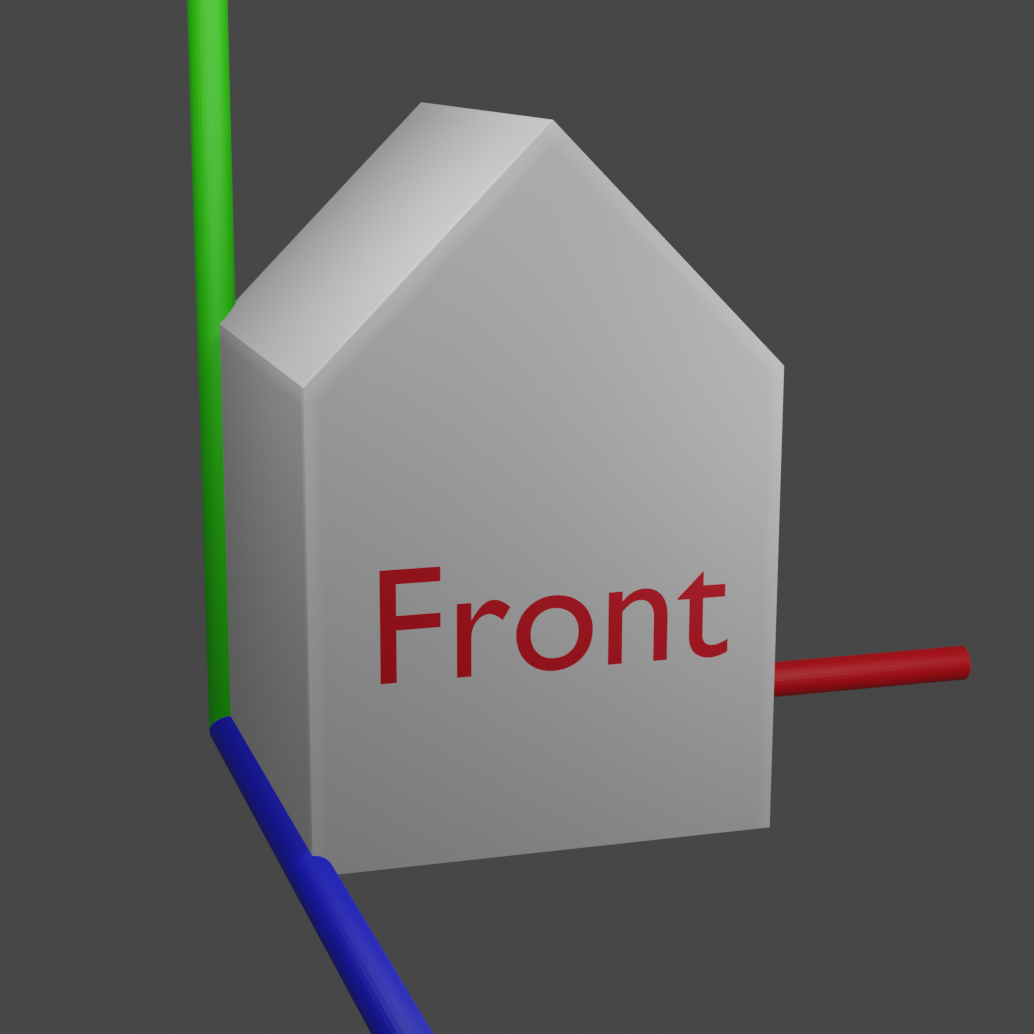
\includegraphics[width = 5cm ]{house_blender.png}}
    \caption{House in blender with drawn axis.}
\end{figure}

I chose the bottom vertex on the rear left of the house as the origin as I would only have to work with positive numbers for the rest of the vertices, and they would also be round numbers (except for the roof) as I am going to make the house with a square base of 1x1. 

Below is a wireframe view of the same house with the coordinates labeled.
\begin{figure}[H]
    \centering
    \fbox{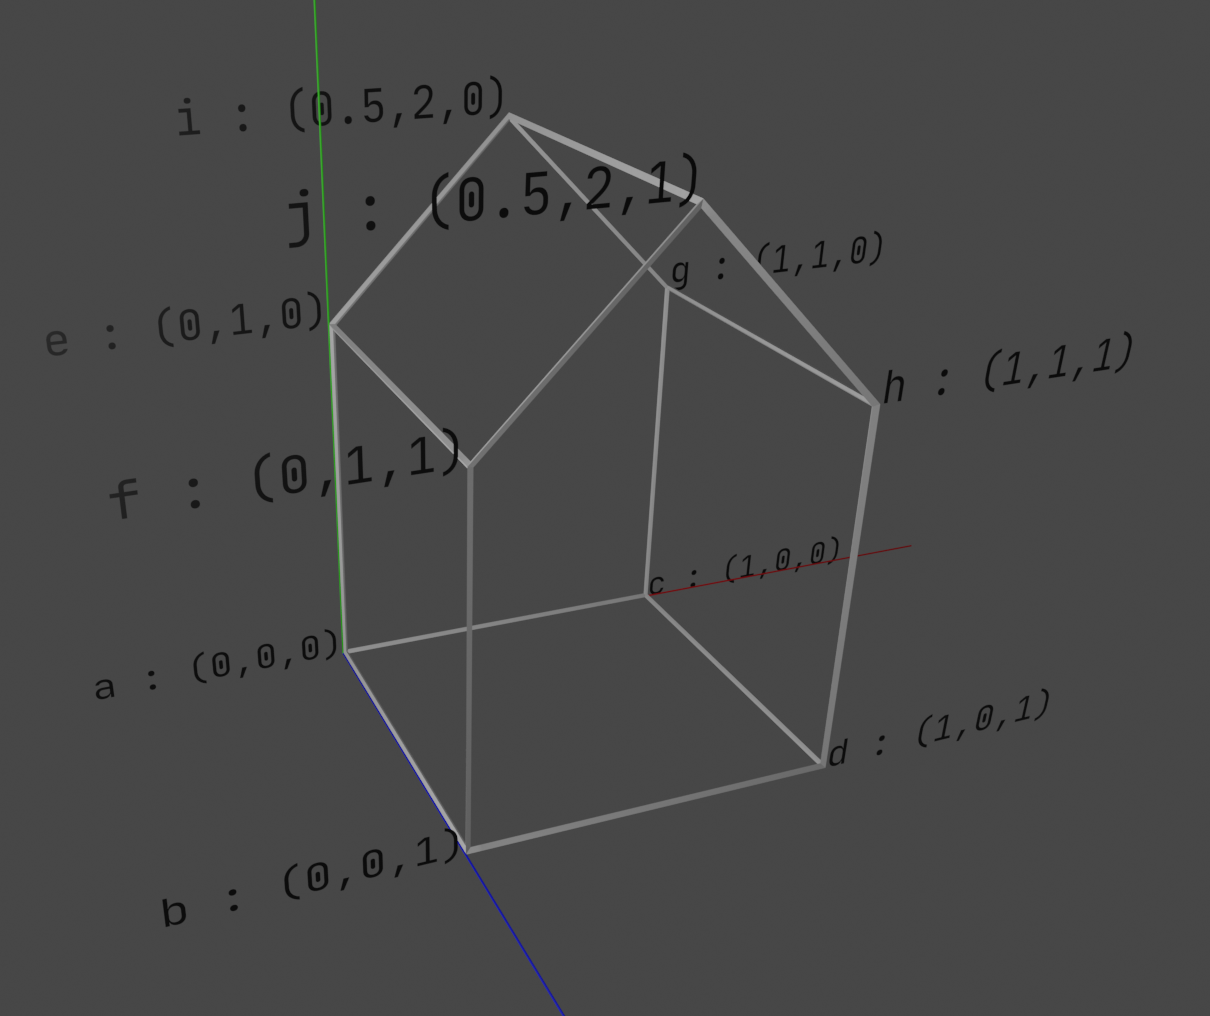
\includegraphics[width = 10cm ]{house_blender_wireframe_with_coord.png}}
    \caption{House in blender with wireframe and coordinates.}
\end{figure}

Coordinates for the vertices:
\begin{enumerate}[(a)]
    \item (0, 0, 0)
    \item (0, 0, 1)
    \item (1, 0, 0)
    \item (1, 0, 1)
    \item (0, 1, 0)
    \item (0, 1, 1)
    \item (1, 1, 0)
    \item (1, 1, 1)
    \item (0.5, 2, 0)
    \item (0.5, 2, 1)
\end{enumerate}

16 triangles will be used to make up the house, and there will be normals that are shared between them.

% \begin{comments}
% Left
% (a, b, f)
% (a, f, e)

% Front
% (b, h, f)
% (b, d, h)
% (f, h, j)

% Right
% (d, g, h)
% (d, c, g)

% Back
% (c, e, g)
% (c, a, e)
% (g, e, i)

% Base
% (a, c, b)
% (b, c, d)

% Roof Left
% (e, j, i)
% (e, f, j)

% Roof Right
% (h, i, j)
% (h, g, i)
% \end{comments}

\section{Normals and OBJ}

I calculated the surface normals by using the following equation:

If we have 3 vectors that make up a a triangle in an anti-clockwise manner: \(V0, V1, V2\), to calculate the normal facing outwards we do:

\(A = V1 - V0\)  |  \(B = V2 - V0\)

\(Normal = A \times B\)

Doing this with the first triangle on the table (triangle on the left face of the house) give you:

\(A = (0, 0, 1) - (0, 0, 0)\) \\ \(A = (0, 0, 1)\)

\(B = (0, 1, 1) - (0, 0, 0)\) \\ \(B = (0, 1, 1)\)

\(Normal = (0, 0, 1) \times (0, 1, 1)\) \\ \(Normal = (-1, 0, 0)\)

I confirmed this calculation to be correct by looking at the shape itself in 3D space, and \((-1, 0, 0)\) is the normal that would be correct.

I had no need to normalise the vectors as they output from the cross product was a sensible number.

Same calculation is done for the rest of the sides, triangles facing the same direction will have the same surface normals.

\begin{table}[H]
    \begin{tabular}{|l|l|} 
    \hline
    \textbf{ Triangles } & \textbf{Normals }              \\ 
    \hline
    (a, b, f)            & \multirow{2}{*}{(-1, 0, 0)}    \\
    (a, f, e)            &                                \\ 
    \hline
    (b, h, f)            & \multirow{3}{*}{(0, 0, 1)}     \\
    (b, d, h)            &                                \\
    (f, h, j)            &                                \\ 
    \hline
    (d, g, h)            & \multirow{2}{*}{(1, 0, 0)}     \\
    (d, c, g)            &                                \\ 
    \hline
    (c, e, g)            & \multirow{3}{*}{(0, 0, -1)}    \\
    (c, a, e)            &                                \\
    (g, e, i)            &                                \\ 
    \hline
    (a, c, b)            & \multirow{2}{*}{(0, -1, 0)}    \\
    (b, c, d)            &                                \\ 
    \hline
    (e, j, i)            & \multirow{2}{*}{(-1, 0.5, 0)}  \\
    (e, f, j)            &                                \\ 
    \hline
    (h, i, j)            & \multirow{2}{*}{(1, 0.5, 0)}   \\
    (h, g, i)            &                                \\
    \hline
    \end{tabular}
\end{table}

I calculated the vertex normals by taking the normals for the triangles that share that vertex, and average the X, Y and Z and then normalised the output.

Working out for vertex (0,0,0):

\(Normals of triangles that share the vertex (0,0,0): (-1,0,0) (0,-1,0) (0,0,-1)\)

\(X Average: -1 + 0 + 0\)

\(Y Average: 0 + -1 + 0\)

\(Z Average: 0 + 0 + -1\)
\( = (-1,-1,-1)\)

\(Normalise  (-1,-1,-1) = 
(-0.57735, -0.57735, -0.57735) (5dp)\)

To write the .obj file, I have to change the alphabetical indices that I have been using into numerical. I have rounded the numbers to 6 decimal places. I have the same number of vertex normals as vertices as I decided to make the shape smooth shaded. 






\begin{enumerate}[v]
    \item 0 0 0 % 1 a
    \item 0 0 1 % 2 b
    \item 1 0 0 % 3 c
    \item 1 0 1 % 4 d
    \item 0 1 0 % 5 e
    \item 0 1 1 % 6 f
    \item 1 1 0 % 7 g
    \item 1 1 1 % 8 h
    \item 0.5 2 0 % 9 i
    \item 0.5 2 1 % 10 j
\end{enumerate}     
% normalize vector (-0.333333333333, -0.333333333333, -0.333333333333)
% normalize vector (-0.333333333333, -0.333333333333, 0.333333333333)
% normalize vector (0.333333333333 ,-0.333333333333,-0.333333333333)
% normalize vector (0.333333333333 ,-0.333333333333,0.333333333333)
% normalize vector (-0.66666666667, 0.1666666667,-0.333333333333)
% normalize vector (-0.66666666667, 0.1666666667,0.333333333333)
% normalize vector (0.0, 0.1666666667, -0.333333333333)
% normalize vector (0.0, 0.1666666667, 0.333333333333)
% normalize vector (0.0, 0.333333333333, -0.333333333333)
% normalize vector (0.0, 0.333333333333, 0.333333333333)
%
% % Un-normlaised
% \begin{enumerate}[vn]
%     \item -0.333333 -0.333333 -0.333333 % 1 a
%     \item -0.333333 -0.333333 0.333333 % 2 b
%     \item 0.333333 -0.333333 -0.333333 % 3 c
%     \item 0.333333 -0.333333 0.333333 % 4 d
%     \item -0.666667 0.166667 -0.333333 % 5 e
%     \item -0.666667 0.166667 0.333333 % 6 f
%     \item 0.0 0.166667 -0.333333 % 7 g
%     \item 0.0 0.166667 0.333333 % 8 h
%     \item 0.0 0.333333 -0.333333 % 9 i
%     \item 0.0 0.333333 0.333333 % 10 j
% \end{enumerate}  

% Normalised
\begin{enumerate}[vn]
    \item -0.57735 -0.57735 -0.57735 % 1 a
    \item -0.57735 -0.57735 0.57735 % 2 b
    \item 0.57735 -0.57735 -0.57735 % 3 c
    \item 0.57735 -0.57735 0.57735 % 4 d
    \item -0.872872 0.218218 -0.436435 % 5 e
    \item -0.872872 0.218218 0.436435 % 6 f
    \item 0 0.447215 -0.894427 % 7 g
    \item 0 0.447215 0.894427 % 8 h
    \item 0 0.707107 -0.707107 % 9 i
    \item 0 0.707107 0.707107 % 10 j
\end{enumerate}  

usemtl matWall
\begin{enumerate}[f]
    \item 1//1 2//2 6//6
    \item 1//1 6//6 5//5
    \item 2//2 8//8 6//6
    \item 2//2 4//4 8//8
    \item 6//6 8//8 10//10
    \item 4//4 7//7 8//8
    \item 4//4 3//3 7//7
    \item 3//3 5//5 7//7
    \item 3//3 1//1 5//5
    \item 7//7 5//5 9//9
    \item 1//1 3//3 2//2
    \item 2//2 3//3 4//4
\end{enumerate}
usemtl matRoof
\begin{enumerate}[f]
    \item 5//5 10//10 9//9
    \item 5//5 6//6 10//10
    \item 8//8 9//9 10//10
    \item 8//8 7//7 9//9
\end{enumerate}


\chapter{Question 2 - Vertex Buffer Object(VBO) design and transformations}

\section{VBO Design}

My single VBO will look like this:
\begin{verbatim}
x y z x y z x y z r g b r g b r g b
\end{verbatim}
which is the standard format, making the attributes tightly packed.

I will add the vertices for the triangles into an array of floats of size = 3 * 3 * numberOfTriangles, three floats per coordinate, 3 coordinates per triangle in the counter-clockwise order they should be drawn to render outside, the first two triangles will look like this followed by the rest of the vertices:

triangleVertices[144] = 

\{0, 0, 0,

0, 0, 1

0, 1, 1,

0, 0, 0,

0, 1, 1,

0, 1, 1,

...\}


As the RGB values are in the VBO, I will initialise them as an array of size 144 as well.

triangleColors[144] = 

\{1, 1, 1,

1, 1, 1,

1, 1, 1,

1, 1, 1,

1, 1, 1,

1, 1, 1, 

...\}


Two uint (GLuint) variables will need to be created, one is VAO (will be called \textbf{vao}) and the other is VBO (will be called \textbf{vbo}).

We then call the following functions:
\begin{lstlisting}[language=c]
    // Will have to create two arrays of floats that contain the vertices for all the triangles and the colours for all the triangles both size 10 
    const GLfloat triangleVertices[144] = {...`will have all the vertices here as floats`...}
    const GLfloat triangleColours[144] = {...`will have all the colour data here as floats`...}

    // Will generate a vertex array object (allocate space) and assign it to vao. We pass through a reference so that it will change the variable.
    glGenVertexArrays(1, &vao);

    // Bind the VAO created to the current object
    glBindVertexArray(vao);

    // We then allocate space and generate a vbo, again passing through a reference
    glGenBuffers(1, &vbo)

    // then bind the vbo to the target which is GL_ARRAY_BUFFER
    glBindBuffer(GL_ARRAY_BUFFER, vbo)

    // We allocate the buffer space required for our data for the VBO
    // the size is 288 as it is sizeof(triangleVertices) + sizeof(triangleColors)
    glBufferData(GL_ARRAY_BUFFER, 288, NULL, GL_STATIC_DRAW);


    // We pass in the data separately by sub-dividing the buffer, as we would like to allocate vertices and color to the same buffer. This could be done so that you create two separate buffers and VBOs like seen on https://www.khronos.org/opengl/wiki/Tutorial2:_VAOs,_VBOs,_Vertex_and_Fragment_Shaders_(C_/_SDL)#Compilation
    // Here, 0 is the starting index and 144 is the sizeof(triangleVertices)
    glBufferSubData(GL_ARRAY_BUFFER, 0, 144, triangleVertices); // vertices
    
    // Here, 144 is the starting index and 144 is the sizeof(triangleColours)
    glBufferSubData(GL_ARRAY_BUFFER, 144, 144, triangleColours); // colours

    // we will enable the vertex attribute arrays one after the other creating the correct 
    glEnableVertexAttribArray(0);
    
    glEnableVertexAttribPointer(0, 3, GL_FLOAT, GL_FALSE, 0, 0);
    
    
    glEnableVertexAttribArray(1);
    // here the last parameter is a pointer to 144 as that is where the colour data starts in the buffer
    glEnableVertexAttribPointer(1, 3, GL_FLOAT, GL_FALSE, 0, (const GLvoid*) 144);

    
\end{lstlisting}

% This should pass the vertex data to a buffer in the GPU.

\section{Transformation and rendering}

Now to transform it and then render the object we will use a glutil::MatrixStack to transform the object.

\begin{lstlisting}[language=c]

    glUtil::MatrixStack matrixStack; // creating the stack
    matrixStack.SetIdentity(); // setting it to an identity matrix

    matrixStack.Push();
        // 14 points on X, 6 Points on Z, so it is still on the ground plane while being on a new positions
        matrixStack.Translate(14, 0, 6);
        // rotating 38 degrees on the y axis
        matrixStack.Rotate(glm::vec3(0, 1, 0), 38);
        // scaling the house by 3.7f uniform points
        matrixStack.Scale(3.7f);


        // now to render the triangles we pass in the vao that we created and the number of triangles * 3 and then draw it on screen.
        glBindVertexArray(vao);
        glDrawElements(GL_TRIANGLES, 48, GL_UNSIGNED_INT, 0)
    matrixStack.Pop();

\end{lstlisting}

\chapter{Question 3 - Camera Positioning}

\section{Description and calls}

\(\textbf{zNear}\) and \(\textbf{zFar}\) define the distance of the near and far clipping planes. Anything that is in front of the camera but its distance is less than \(\textbf{zNear}\), it will not be displayed; vice versa with \(\textbf{zFar}\), anything in front of the camera but farther away than \(\textbf{zFar}\) will not be shown.

\(\textbf{fovy}\) is the field of view of the camera, giving a bigger number will increase the field of view and display more on screen, decreasing it will compress the image and only show a little portion of it. It is the angle $\theta$ of the separation of the planes on the Y axis. See image I created below that shows it better.

\begin{figure}[H]
    \centering
    \fbox{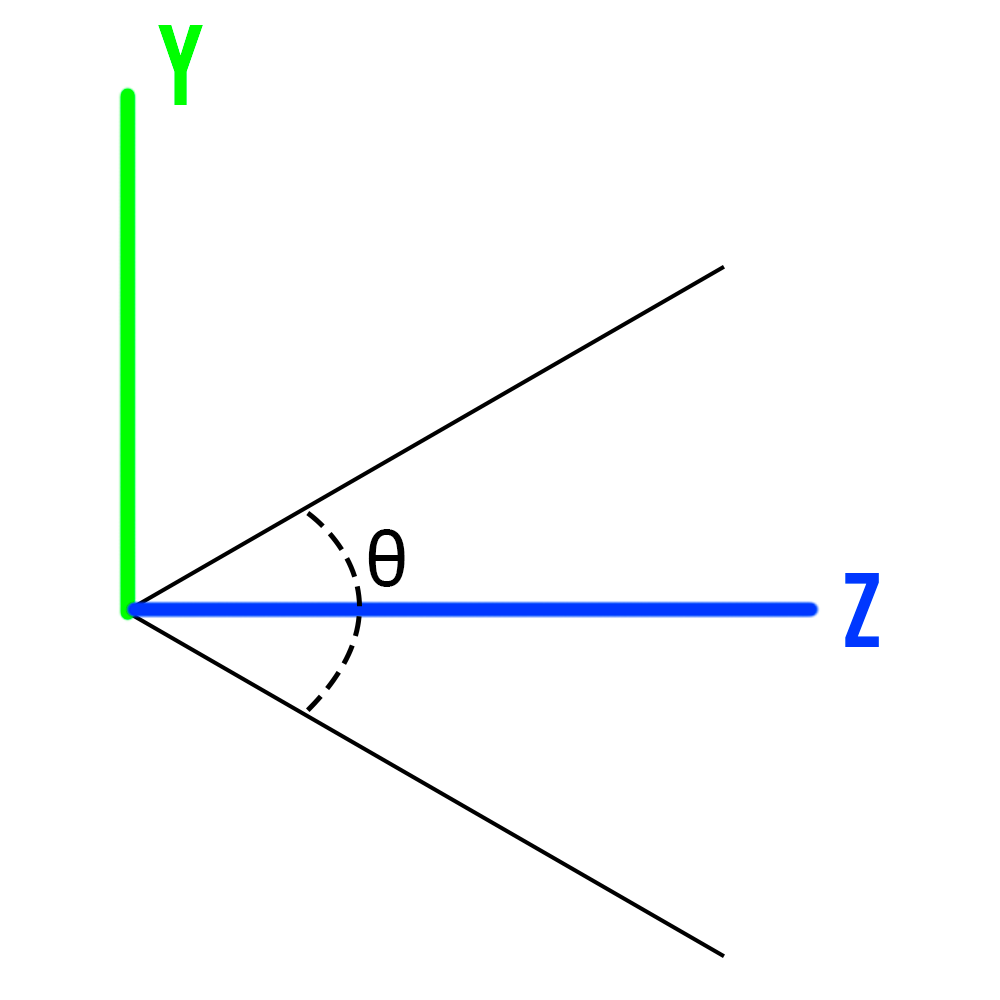
\includegraphics[width = 10cm ]{FOV.png}}
    \caption{Diagram showing what the FOV number/angle means. In this image the two lines are 60$^{\circ}$ apart}
\end{figure}

The \(\textbf{aspect}\) is the ratio between the width (x) and the height (y) of the view, it can also be described as the field of view in the X axis.

Calling \(gluPerspective()\) with these parameters (which are all of type GLdouble) will set up a perspective projection matrix.

I will use the original position for house as seen in question 1 and not the position transformed to in question 2.

I will have the camera's perspective projection matrix be created with the following parameters: 
\begin{lstlisting}[language = c]
    fovy = 60.0 // an appropriate angle that is similar to the human eye
    aspect = 1 // making it square
    zNear = 1 // I do not want objects in front of the camera to clip to early
    zFar = 50 // plenty of room for the far end of the clipping plane.
\end{lstlisting}

Now to position the camera and provide the forward and the up vector. I will position it so that the camera is pointing straight into it and looking at the front of the house.
\begin{lstlisting}[language = c]
    // The house is sitting on the XZ plane and has a total height of 2, so I placed the camera on the center with 1 on the Y axis. As the house goes from 0 to 1 on the X, I decided to place the camera in the center, this being 0.5. As the house already extrudes by 1 on the Z axis, I moved the camera back by 2 extra points to make sure that the house will fit into the FOV, making it 3 on the Z.

    cameraPosition = glm::vec3(0.5f, 1, 3) 

    // the forward is -1 on the Z as it is facing the front of the house that has a normal of (0,0,1)
    cameraForward = glm::vec3(0,0,-1) 

    // the up is going to be positive on the Y as the camera is not angled.
    cameraUp = glm::vec3(0,1,0) 
\end{lstlisting}

\section{Moving the camera around the house}
There are two methods of rotating the camera around a certain object while always keeping it in the center of view.
One is by creating a Catmull Rom Spline that is a circle around the house.

The other is using sin and cos (using a trig unit circle) over delta time to get the correct positions of X and Z. I will be going with the later method as it seems the most straight forward.

\begin{figure}[H]
    \centering
    \fbox{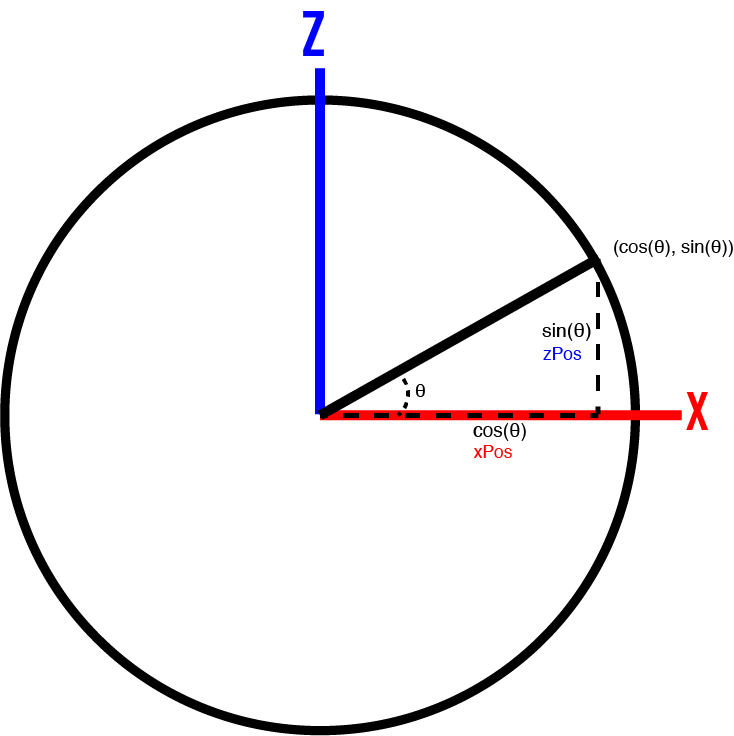
\includegraphics[width = 10cm ]{Trig_Circle.png}}
    \caption{Diagram explaining using the trig unit circle finding out the x and z positions}
\end{figure}


We can use the glm::lookAt() method to get a viewing matrix that will change what is being seen in the world. The following code will be executed every frame, and am assuming delta time \(dt\) is being passed through. The radius will be 10 in this case, and will be offset by the house's position.

\begin{lstlisting}[language = c]
    // set the radius
    radius = 10

    // the height from the house that the camera will be placed at
    auto yPos = 1 + house.position.y // offset by the house's Y

    // house.position is a vec3 with the house's position
    // get the X position 
    auto xPos = (cos(dt) * radius) + house.position.x; // offset by house's X

    // get the Z position
    auto zPos = (sin(dt) * radius) + house.position.z; // offset by house's Z

    cameraPosition = glm::vec3(xPos, yPos, zPos); // will be the vEye in the lookAt

    cameraUp = glm::vec3(0,1,0); // will be the camera up variable

    // updating the view matrix with the new camera data
    // lookAt(eyePosition, viewPoint, cameraUpVector)
    viewMatrix = glm::lookAt(cameraPosition, house.position, cameraUp);

\end{lstlisting}


\chapter{Question 4 - Shader Implementation}

Below is what the 2 shader files will look like. One vertex shader, adn another fragment shader.

\begin{lstlisting}[language = c]
/* shader.vert */
    
    // This is passed in through the client program
    // These matrices describe how the shape will be transformed.
    uniform struct Matrices{
        mat4 projMatrix;
        mat4 modelViewMatrix;
    } matrices;

    // position is passed in to first location
    // this first location is the first location of the vertex buffer from the vao which contained the x y z
    layout(location = 0) in vec3 inPosition;

    // colour is passed through to the second location
    // this second location is the second location of the vertex buffer from the vao which contains the r g b
    layout(location = 1) in vec3 inColour;

    out vec3 color

    void main(){
        // the position is altered by the matrix that is passed in
        gl_Position = matrices.projMatrix * matrices.modelViewMatrix * vec4(inPosition, 1.0f);

        // the colour from the VBO is passed out to the fragment shader
        color = inColour;
    }
\end{lstlisting}

\begin{lstlisting}[language = c]
/* shader.frag */ 

    // colour is passed in from the vertex shader.
    in vec3 colour;
    // frag colour is output
    out vec4 fragColour;
    void main(){
        // the colour of the fragment is the changed to the colour that is passed in via the client via the vertex shader
        fragColour = vec4(fragColour 1.0);
    }

\end{lstlisting}

Below is the same code from 2.2 in the client program (render method) however with the setting the  uniforms.

\begin{lstlisting}
    glUtil::MatrixStack matrixStack; // creating the stack
    matrixStack.SetIdentity(); // setting it to an identity matrix

    matrixStack.Push();
        matrixStack.Translate(14, 0, 6);
        matrixStack.Rotate(glm::vec3(0, 1, 0), 38);
        matrixStack.Scale(3.7f);

        // we pass in the camera's projection matrix to the shader program
        shaderProgram->SetUniform("matrices.projMatrix", camera->GetPerspectiveProjectionMatrix());

        // we pass in the transformations done using the matrixStack to the shader program
        shaderProgram->SetUniform("matrices.modelViewMatrix", matrixStack.Top());

        // Rendering 
        glBindVertexArray(vao);
        glDrawElements(GL_TRIANGLES, 48, GL_UNSIGNED_INT, 0)
    matrixStack.Pop();

\end{lstlisting}


\chapter{Question 5 - Texture Mapping}

\section{Texture and texture coordinates with OBJ explanation}

Values from Question 1:
Coordinates for the vertices:
\begin{enumerate}[(1)]
    \item (0, 0, 0) % 1 a
    \item (0, 0, 1) % 2 b
    \item (1, 0, 0) % 3 c
    \item (1, 0, 1) % 4 d
    \item (0, 1, 0) % 5 e
    \item (0, 1, 1) % 6 f
    \item (1, 1, 0) % 7 g
    \item (1, 1, 1) % 8 h
    \item (0.5, 2, 0) % 9 i
    \item (0.5, 2, 1) % 10 j
\end{enumerate}

Below is the the image of the texture I will be using, I decided to place both roof and walls onto the same texture image and then give coordinates separately, as this avoids having to load 2 images, both materials will use the same texture.

\begin{figure}[H]
    \centering
    \fbox{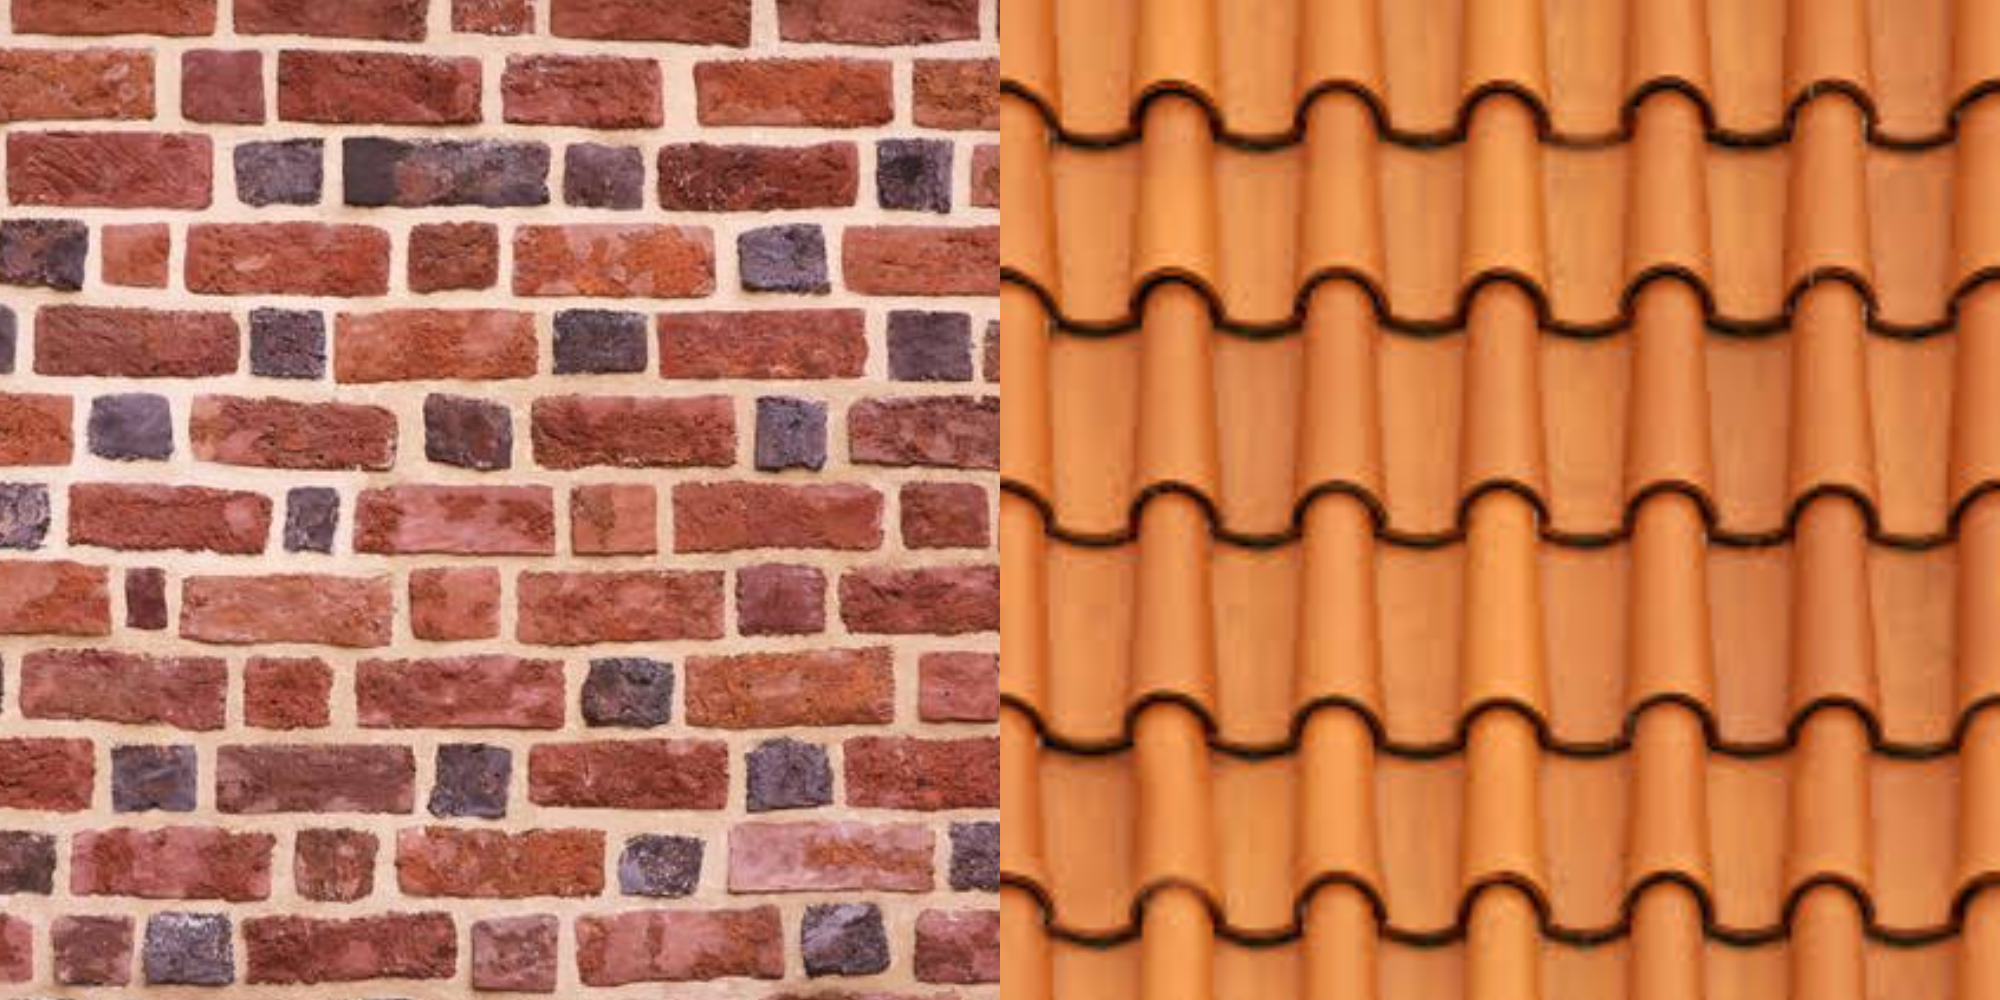
\includegraphics[width = 5cm ]{texturemap.png}}
    \caption{Image of the texture I will be using.}
\end{figure}

The coordinates of the texture are broken down like the following diagram.
\begin{figure}[H]
    \centering
    \fbox{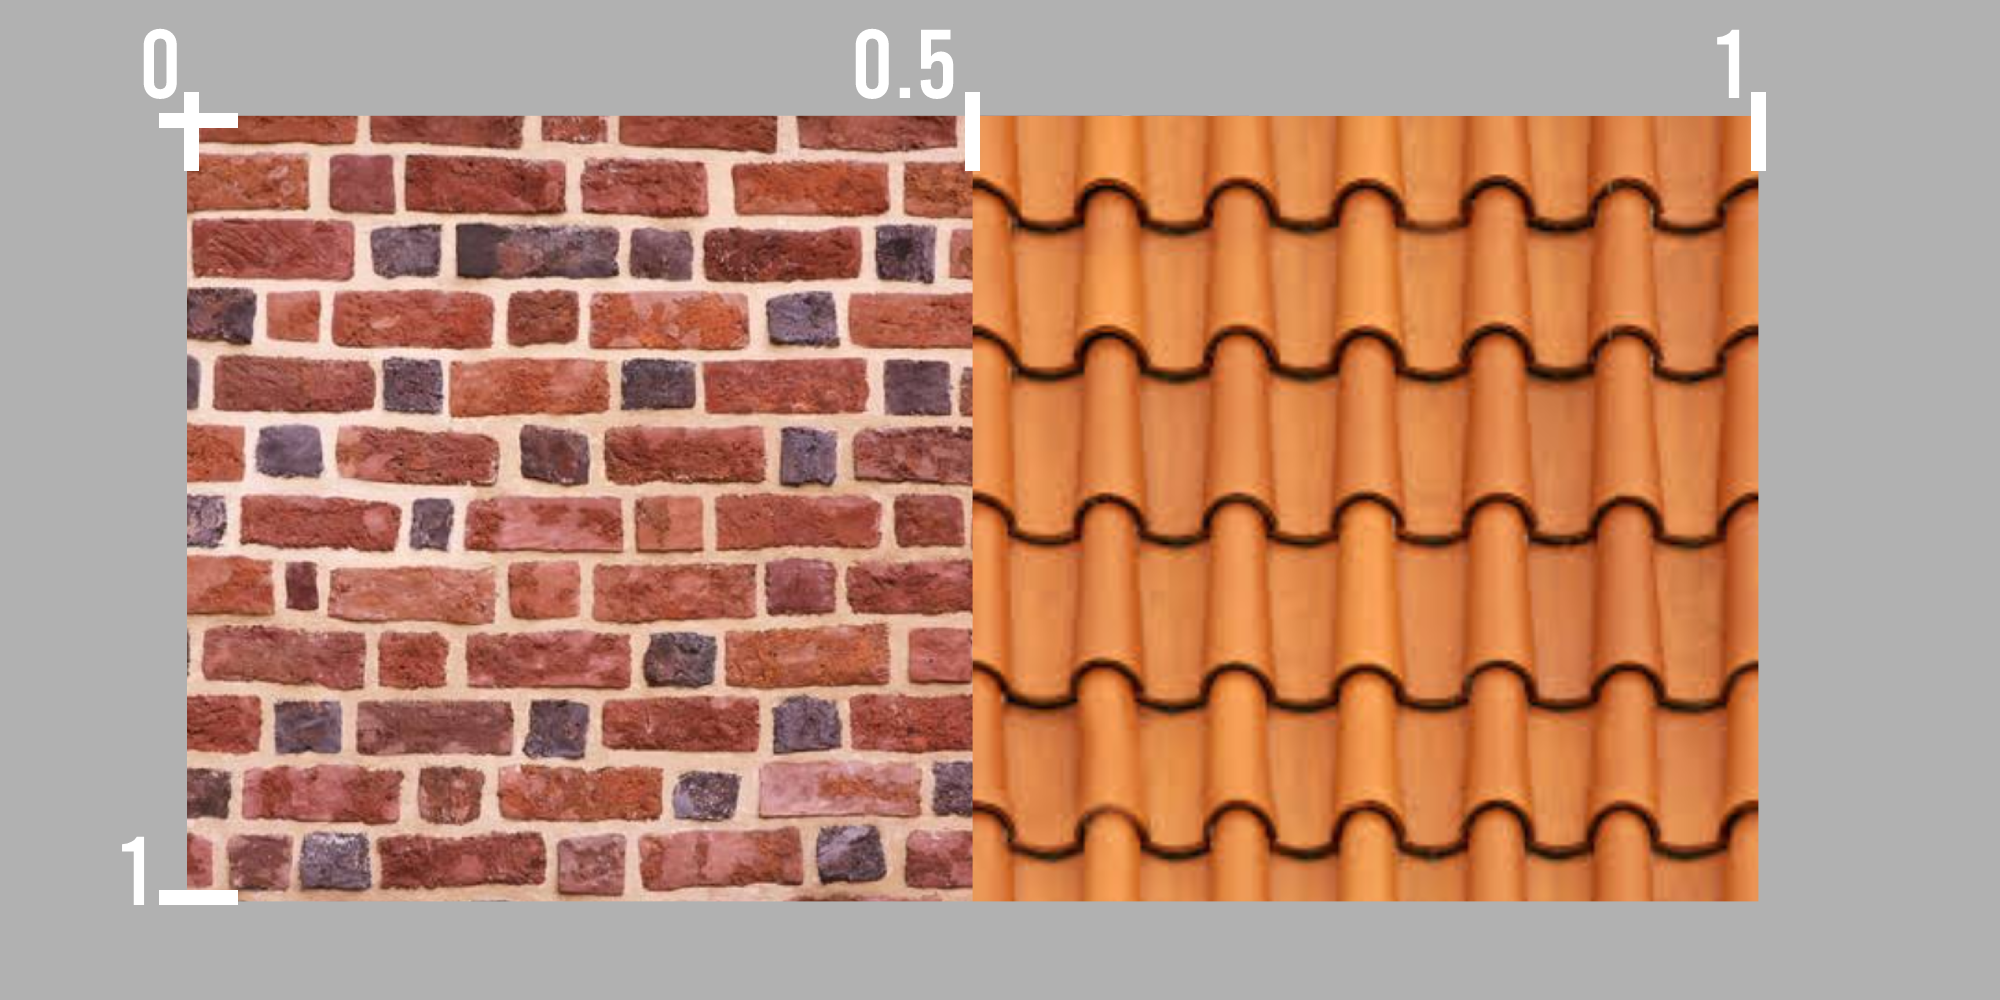
\includegraphics[width = 5cm ]{texturemap_labelled.png}}
    \caption{Coordinates marked on texture image.}
\end{figure}

I will break the texture down into two triangles each like below. (Note these triangles could be oriented the other way using the same coordinates)
\begin{figure}[H]
    \centering
    \fbox{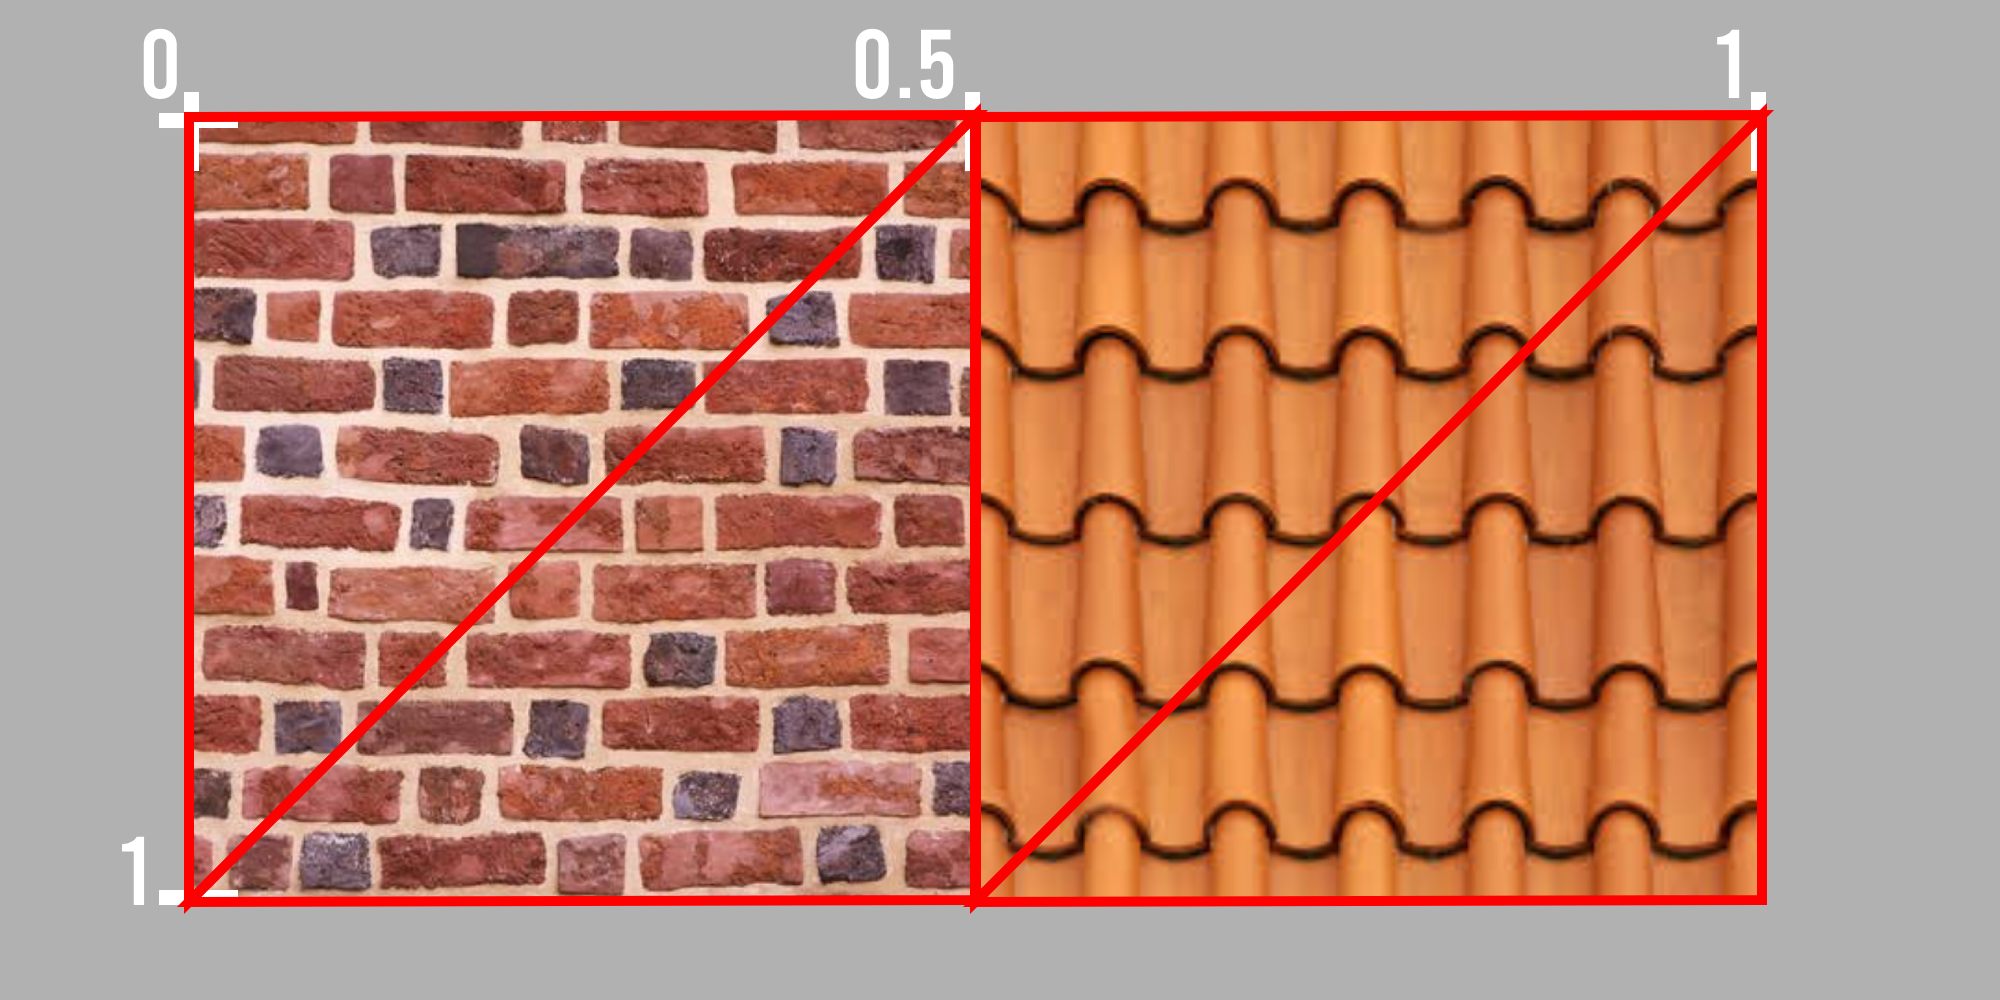
\includegraphics[width = 5cm ]{texturemap_triangles.png}}
    \caption{Texture split into triangles}
\end{figure}


Texture Coordinates
\begin{enumerate}[(1)]
    \item (0, 0)
    \item (0, 1)
    \item (0.5, 0)
    \item (0.5, 1)
    \item (1, 0)
    \item (1, 1)
\end{enumerate}

Now as an Obj file to show the texture coordinates per vertex of the triangles. Will be represented as v/vt/vn. 

Note: The triangles (6,8,10) and (7,5,9) are considered parts of the wall and not the roof, only the slant is considered the roof.

Below is appended after the vertices are listed.
\begin{enumerate}[vt ]
    \item 0 0  % 1
    \item 0 1  % 2
    \item 0.5 0  % 3
    \item 0.5 1  % 4
    \item 1 0  % 5
    \item 1 1  % 6
\end{enumerate}

The below is an amendment to the faces.
% \begin{enumerate}[(1)]
%     \item (0, 0, 0) % 1 a
%     \item (0, 0, 1) % 2 b
%     \item (1, 0, 0) % 3 c
%     \item (1, 0, 1) % 4 d
%     \item (0, 1, 0) % 5 e
%     \item (0, 1, 1) % 6 f
%     \item (1, 1, 0) % 7 g
%     \item (1, 1, 1) % 8 h
%     \item (0.5, 2, 0) % 9 i
%     \item (0.5, 2, 1) % 10 j
% \end{enumerate}

usemtl matWall
\begin{enumerate}[f]
    \item 1/2/1 2/4/2 6/3/6
    \item 1/2/1 6/3/6 5/1/5
    \item 2/4/2 8/3/8 6/1/6
    \item 2/1/2 4/4/4 8/3/8
    \item 6/2/6 8/3/8 10/1/10
    \item 4/2/4 7/3/7 8/1/8
    \item 4/2/4 3/4/3 7/3/7
    \item 3/2/3 5/3/5 7/1/7
    \item 3/2/3 1/4/1 5/3/5
    \item 7/2/7 5/3/5 9/1/9
    \item 1/3/1 3/1/3 2/4/2
    \item 2/4/2 3/1/3 4/2/4
\end{enumerate}
usemtl matRoof
\begin{enumerate}[f]
    \item 5/4/5 10/5/10 9/3/9
    \item 5/4/5 6/6/6 10/5/10
    \item 8/4/8 9/5/9 10/3/10
    \item 8/4/8 7/6/7 9/5/9
\end{enumerate}


% TODO GLSL code
\section{VBO design}
The VBO design will need to be altered to make room for the texture coordinates in the buffer. Because the textures only have 2 coordinates, I will make the size of one vertex 2 floats.

When I create the triangleVertices and triangleColors, I will also create triangleTextures that will be of size 2 $\times$ 3 $\times$ numberOfTriangles: 

The first two triangles will look like this:
\begin{verbatim}
    triangleTextures[96] = 
    {0 , 1,
    0.5, 1,
    0.5, 0,
    0, 1,
    0.5, 0,
    0, 0,
    ...}
\end{verbatim}

The VBO will look like this: x y z x y z x y z r g b r g b r g b u v u v u v 

We will have to allocate more space to the buffer for the triangles, and will have to split it into another sub buffer data and enable that.

\begin{lstlisting}[language=c]
    // first we create the array just under triangleVertices and triangleColours
    const GLfloat triangleTextures[96] = {...`will have all the colour data here as floats`...}

    ...

    // this will replace the previous glBufferData call.
    // the size is 384 as it is sizeof(triangleVertices) + sizeof(triangleColors) + sizeof(triangleTextures)
    glBufferData(GL_ARRAY_BUFFER, 384, NULL, GL_STATIC_DRAW);

    ...

    // after the calls to create sub buffers we create another bufferSubData for the textures
    // Here, 288 is the starting index and 96 is the sizeof(triangleTextures) 
    glBufferSubData(GL_ARRAY_BUFFER, 288, 144, triangleTextures); // textures

    ...

    // we enable the vertex attribute after activating the others
    glEnableVertexAttribArray(2);
    // the index is 2, there are 2 floats per vertex, and the size is 96
    glEnableVertexAttribPointer(2, 2, GL_FLOAT, GL_FALSE, 0, (const GLvoid*) 96);

\end{lstlisting}

\section{Door and four windows}

\subsection{Using Texture}

I would render the house by just changing the texture by changing the texture into the following: and then using the section with the doors and widows for only the front of the house.

\begin{figure}[H]
    \centering
    \fbox{\includegraphics[width = 10cm ]{texture_doorsWindows.png}}
    \caption{Texture with doors and windows}
\end{figure}

\begin{figure}[H]
    \centering
    \fbox{\includegraphics[width = 10cm ]{texture_doorsWindows_labbleed.png}}
    \caption{Texture with doors and windows labelled}
\end{figure}


This change in texture will lead to the coordinates changing in the OBJ file, the indices needn't change however more will be added. Then in the triangles for the front of the house the right most texture will be used.


I will describe it using changes to be made to the OBJ file:

Below is appended after the vertices are listed.
\begin{enumerate}[vt ]
    \item 0 0  % 1
    \item 0 1  % 2
    \item 0.33333 0  % 3
    \item 0.33333 1  % 4
    \item 0.66667 0  % 5
    \item 0.66667 1  % 6
    \item 1 0 % 7
    \item 1 1 % 8
\end{enumerate}

Only change to be made to the faces section is the texture indices for the front face.

This: 

\dots
\begin{enumerate}[f]
    \item 2/4/2 8/3/8 6/1/6
    \item 2/1/2 4/4/4 8/3/8
\end{enumerate}
\dots

will change into:

\dots
\begin{enumerate}[f]
    \item 2/6/2 8/7/8 6/5/6
    \item 2/6/2 4/8/4 8/7/8
\end{enumerate}
\dots


This will keep all the other textures the same but change the front of the house.

\subsection{Using Geometry}

We can change the geometry of the front of the house to make it have triangles for the door, window and wall, doing this will create many triangles as this is going to be one face and not separate shapes.

Below is the diagram I created which shows how I went about splitting the shape into the least amount of triangles possible.

\begin{figure}[H]
    \centering
    \fbox{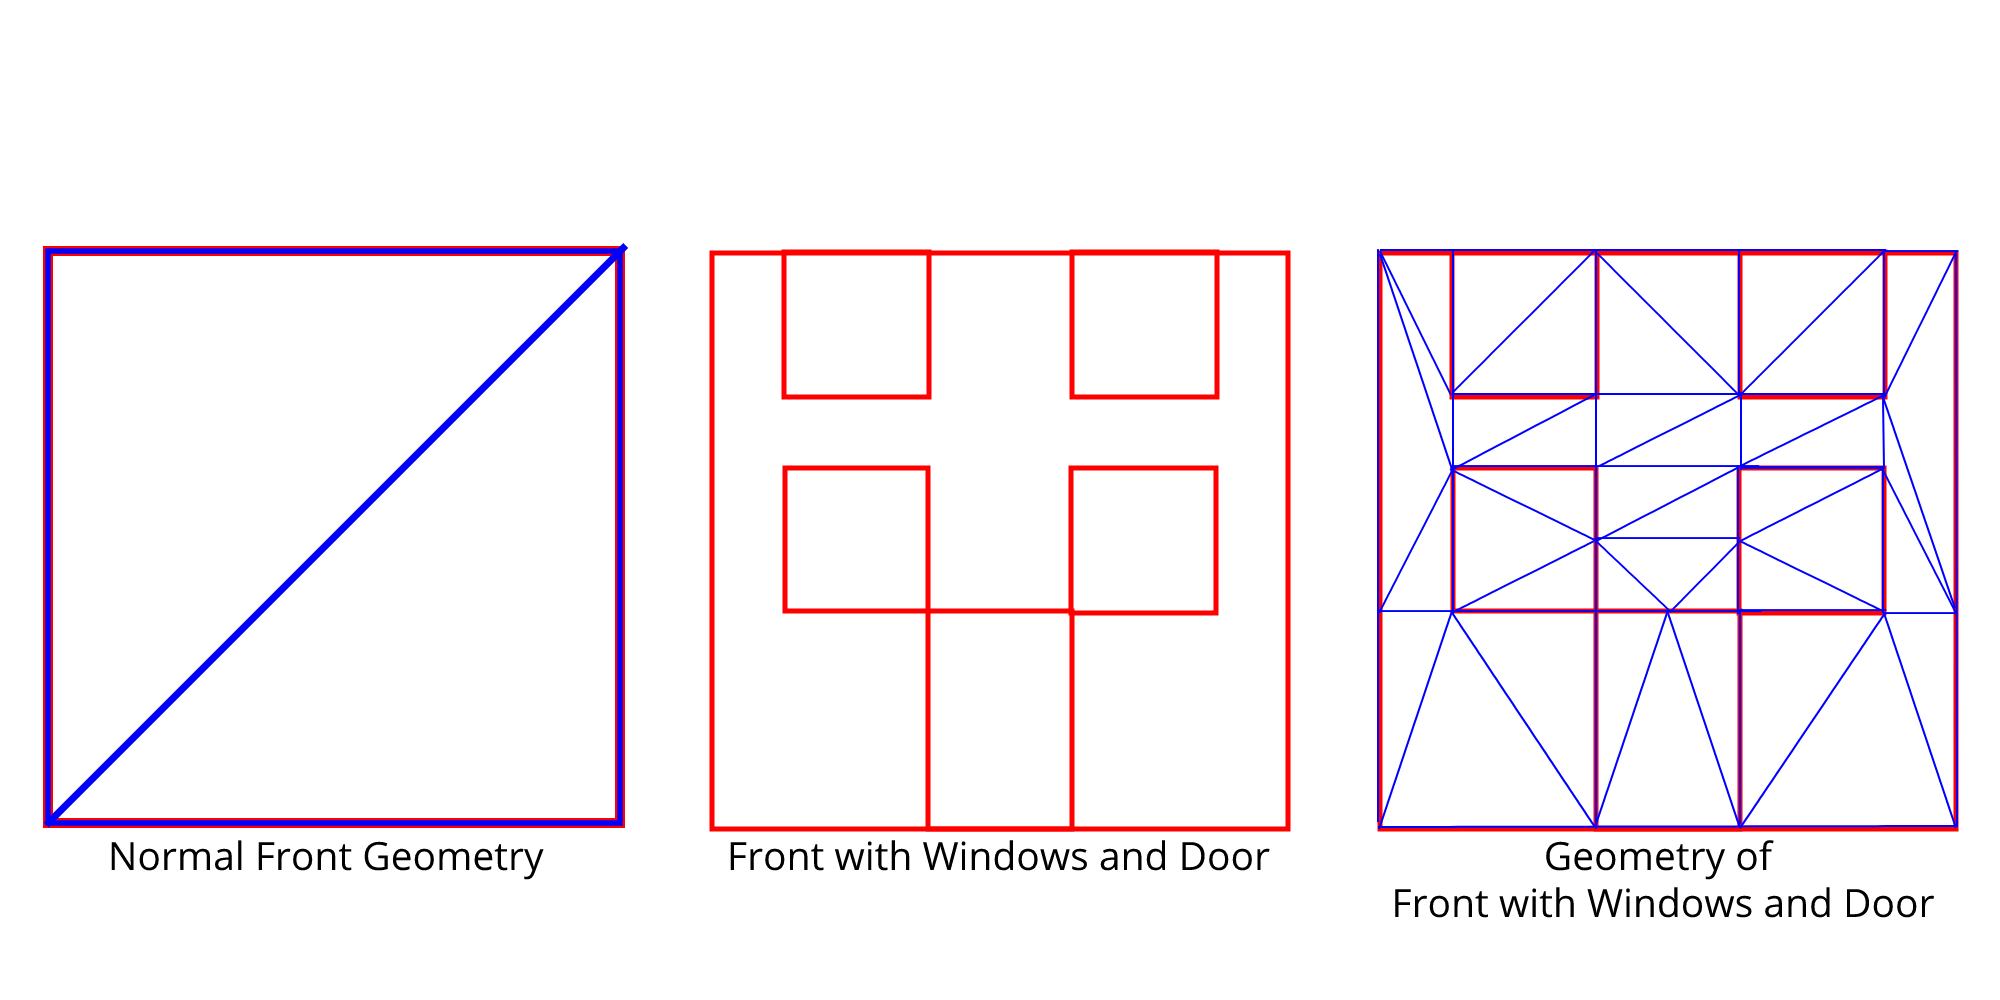
\includegraphics[width = 10cm ]{geometry_windwos.png}}
    \caption{Geometry of the front of the house broken down.}
\end{figure}

This accounts to having 40 triangles for the shape; and 26 vertices. The 13 triangles inside of the door and windows will have different colour vectors to the rest of the house. 


\end{document}